\newcommand{\svcourse}{CST Part IA: Software Engineering and Security}
\newcommand{\svnumber}{1}
\newcommand{\svvenue}{Microsoft Teams}
\newcommand{\svdate}{2022-05-11}
\newcommand{\svtime}{15:00}
\newcommand{\svuploadkey}{CBd13xmL7PC1zqhNIoLdTiYUBnxZhzRAtJxv/ytRdM1r7qIfwMsxeVwM/pPcIo8l}

\newcommand{\svrname}{Dr Sam Ainsworth}
\newcommand{\jkfside}{oneside}
\newcommand{\jkfhanded}{yes}

\newcommand{\studentname}{Harry Langford}
\newcommand{\studentemail}{hjel2@cam.ac.uk}


\documentclass[10pt,\jkfside,a4paper]{article}

% DO NOT add \usepackage commands here.  Place any custom commands
% into your SV work files.  Anything in the template directory is
% likely to be overwritten!

\usepackage{fancyhdr}

\usepackage{lastpage}       % ``n of m'' page numbering
\usepackage{lscape}         % Makes landscape easier

\usepackage{verbatim}       % Verbatim blocks
\usepackage{listings}       % Source code listings
\usepackage{graphicx}
\usepackage{float}
\usepackage{epsfig}         % Embed encapsulated postscript
\usepackage{array}          % Array environment
\usepackage{qrcode}         % QR codes
\usepackage{enumitem}       % Required by Tom Johnson's exam question header

\usepackage{hhline}         % Horizontal lines in tables
\usepackage{siunitx}        % Correct spacing of units
\usepackage{amsmath}        % American Mathematical Society
\usepackage{amssymb}        % Maths symbols
\usepackage{amsthm}         % Theorems

\usepackage{ifthen}         % Conditional processing in tex

\usepackage[top=3cm,
            bottom=3cm,
            inner=2cm,
            outer=5cm]{geometry}

% PDF metadata + URL formatting
\usepackage[
            pdfauthor={\studentname},
            pdftitle={\svcourse, SV \svnumber},
            pdfsubject={},
            pdfkeywords={9d2547b00aba40b58fa0378774f72ee6},
            pdfproducer={},
            pdfcreator={},
            hidelinks]{hyperref}

\renewcommand{\headrulewidth}{0.4pt}
\renewcommand{\footrulewidth}{0.4pt}
\fancyheadoffset[LO,LE,RO,RE]{0pt}
\fancyfootoffset[LO,LE,RO,RE]{0pt}
\pagestyle{fancy}
\fancyhead{}
\fancyhead[LO,RE]{{\bfseries \studentname}\\\studentemail}
\fancyhead[RO,LE]{{\bfseries \svcourse, SV~\svnumber}\\\svdate\ \svtime, \svvenue}
\fancyfoot{}
\fancyfoot[LO,RE]{For: \svrname}
\fancyfoot[RO,LE]{\today\hspace{1cm}\thepage\ / \pageref{LastPage}}
\fancyfoot[C]{\qrcode[height=0.8cm]{\svuploadkey}}
\setlength{\headheight}{22.55pt}


\ifthenelse{\equal{\jkfside}{oneside}}{

 \ifthenelse{\equal{\jkfhanded}{left}}{
  % 1. Left-handed marker, one-sided printing or e-marking, use oneside and...
  \evensidemargin=\oddsidemargin
  \oddsidemargin=73pt
  \setlength{\marginparwidth}{111pt}
  \setlength{\marginparsep}{-\marginparsep}
  \addtolength{\marginparsep}{-\textwidth}
  \addtolength{\marginparsep}{-\marginparwidth}
 }{
  % 2. Right-handed marker, one-sided printing or e-marking, use oneside.
  \setlength{\marginparwidth}{111pt}
 }

}{
 % 3. Alternating margins, two-sided printing, use twoside.
}


\setlength{\parindent}{0em}
\addtolength{\parskip}{1ex}

% Exam question headings, labels and sensible layout (courtesy of Tom Johnson)
\setlist{parsep=\parskip, listparindent=\parindent}
\newcommand{\examhead}[3]{\section{#1 Paper #2 Question #3}}
\newenvironment{examquestion}[3]{
\examhead{#1}{#2}{#3}\setlist[enumerate, 1]{label=(\alph*)}\setlist[enumerate, 2]{label=(\roman*)}
\marginpar{\href{https://www.cl.cam.ac.uk/teaching/exams/pastpapers/y#1p#2q#3.pdf}{\qrcode{https://www.cl.cam.ac.uk/teaching/exams/pastpapers/y#1p#2q#3.pdf}}}
\marginpar{\footnotesize \href{https://www.cl.cam.ac.uk/teaching/exams/pastpapers/y#1p#2q#3.pdf}{https://www.cl.cam.ac.uk/\\teaching/exams/pastpapers/\\y#1p#2q#3.pdf}}
}{}


\usepackage{multicol}
\usepackage{xcolor}
\usepackage{qtree}
\usepackage{float}
\usepackage{graphicx}

\lstdefinestyle{cstyle}{
  belowcaptionskip=1\baselineskip,
  breaklines=true,
  xleftmargin=\parindent,
  language=C,
  showstringspaces=false,
  basicstyle=\footnotesize\ttfamily,
  keywordstyle=\bfseries\color{orange!80!black},
  commentstyle=\itshape\color{purple!40!black},
  identifierstyle=\color{blue},
  stringstyle=\color{green!40!black},
}

\begin{document}

\begin{enumerate}

\item How do software engineering tools change as systems scale?
Discuss this question with reference to:

\begin{enumerate}[label=(\alph*)]

\item A 2000-line device driver for a safety-critical sensor on board an aircraft.

Our primary concerns in this system are quality, performance and correctness.
Due to the size of the system, managing complexity is not a huge concern, however
we should still use some tools to simplify development.

\subsubsection*{Code Quality}

We should firstly note that the system is only 2000 lines large.
This means that all users will have a pretty good understanding of all aspects of the project.
This is good for code quality.
Although highest quality can be obtained by making people work on very similar parts at which they are a specialist.
However, given the safety-critical nature of the project, we should take more precautions to ensure high code quality.
This should include documenting code and following best coding practices \dag.
Programmers should also document their code properly, and review other programmers code regularly. This will minimise
the number of bugs. The programmers should also use IDEs which have error highlighting.
More powerful static analysis tools such as Coverity should also be used (given the importance of this system) .
Static analysis can be used to find errors such as memory leaks or dereferences of NULL pointers.

We can use git with gerrit to mean that other people check over code before it's submitted into the main project.
This is suitable since everyone knows what the code should do.
This means that the programmers will know the whole system well and can use it all properly.
We should use good coding practices.
We can ensure we're doing this by using code analysis tools like Coverity -- which will suggest
do everything from picking up on memory leaks and telling us not to use goto.

\dag \ For example having good control flow by not using ``goto'', only using things with absolutely defined
behaviour and writing code which is obvious to understand.

For example not swapping variables by using:

\begin{lstlisting}[style=cstyle,label={lst:swap_no_temp}]
int main(){
  int a = 12342;
  int b = 2384783;
  a = a ^ b;
  b = a ^ b;
  a = a ^ b;
}
\end{lstlisting}

\subsubsection*{Performance}

This system is safety-critical and (presumably) real-time.
As such, we must take all reasonable efforts to make guarantees about execution time and make the code execute as
fast as possible.
To this end, I would recommend programming in C or C++ instead of a higher level language.
Modern C compilers such as gcc are highly optimised and will compile to optimised
machine code anyway. Note that we should use \textit{modern} compilers.
If the code was highly critical, then programming in assembly (or at worse machine code)
may be appropriate; although the massively increased difficulty in programming due to
``accidental complexity'' usually greatly outweighs the performance gain -- so this is only
recommended for small pieces of code for cases where no language brings the required
speed.

For any computation tasks, we should use libraries rather than write code ourselves.

\subsubsection*{Correctness}

As with every system, we should test this extensively.
There are a number of ways we could do this: for example with test-driven-development.
This enables us to establish success criteria before the project starts.
However, the downside of test-driven-development is that prior to writing the program
we don't know the control flow and might not know all edge-cases.
This means that we may not test all code.

We should also consider are white-box testing - where we know exactly how the program
works and test every thread of execution.

Lastly, we should start ``fuzzing'' -- this is where we generate a large amount of test cases randomly
and pass the system almost every conceivable input and check that the output is correct.
Fuzzing can usually find all reasonable errors in systems.

However any set of test cases does not cover the whole set of possible inputs and input orders over the entire
lifetime of an aircraft.
This means that it's not been (and cannot be) empirically proven that the system will never fail on a
set of inputs.

Given the safety-critical nature of the sensor, we may consider a more extreme measure: proving the code correct.
The Isabelle automated Theorem Prover could be used to prove lemmas about certain parts of the code correct.
This method of proof is tedious but gives guarantees of correctness (of the parts we prove) .
Proving small systems correct is not novel.
As an extreme example; the Sel4 microkernel (containing 6700 lines of C) was proven functionally correct in 2009.
Although proving the entire driver correct would be tedious and (past a certain point) practically pointless,
we should consider proving core parts of it correct and proving more general lemmas such as ``not crashing during
flight'' about the rest of the system.

\subsubsection*{Managing Complexity}

2000 lines is a few weeks work for a team of programmers (potentially less if code can
be re-used from elsewhere -- although this would require careful checks).
In this system, the main way of managing complexity will be to segment the device driver into
several files -- each of which provide a simple interface. The device driver should also be stored in an online
repository such as GitHub to allow users to see everyone else's code and backtrack if errors are introduced.
Since the system is so small, we don't need to have more advanced ways.

\item A 100,000-line engine control unit for a diesel engine that adapts it for use in trucks, 
generators or irrigation pumps.

The tools available are similar to those above. We should exploit static analysis throughout,
use an online repository, code review tools to allow fellow programmers to check
each others code. We should use a higher level language to reduce the
accidental complexity \dag -- the inherent complexity of this system cannot be dealt with.
The design of the software implies that it may be extended greatly in the future --
we should anticipate this fully document our code.
Once again, programmers should use IDEs and follow best coding practices.

The requirements for this controller are not as safety-critical as for the driver, so I would
not recommend \textit{proving} it correct -- although rigorous testing of all components
(including fuzzing) is recommended.

\dag \ Systems such as this often run on very poor hardware -- this may prevent us from using
modern languages. We may also find parts of the code which are time critical and require
programming in a lower level language. But once more, this is not recommended for anything
which is not \textit{highly} time critical. Since the hardware is so niche, we may consider
making some custom hardware -- I won't elaborate since this question asks us to discuss
software engineering tools.

\item A 1,000,000-line social networking site such as Facebook or MySpace.

With this system, the primary concern is managing complexity. Since the system is not safety-critical, we don't need
high assurances of correctness.

\subsection*{Specification}

Figuring out everything which the system should do is a massive task. We should hire a separate team of design
specialists to figure out the full specification before even starting the project.
With large tasks such as this we should employ the waterfall model. This will give every software team a
clear idea of what they should be doing.

\subsection*{Managing Complexity}

The most obvious took for making the project simpler is high level languages. If we write in low level languages (or
languages with fewer features) then lots of effort is spent ``fighting'' the language. The development process can be
made significantly easier if we choose to use a high level language for most of the system. For this particular
application, I would recommend Java or Kotlin. Using either of these languages (with a suitable IDE) would make the
system significantly easier. However, we must note that both are much slower than writing in a lower level language.
Speed doesn't matter so much in this application (and in cases where it does we can interface to a faster language
when required). Modern compilers are fairly efficient and remove almost all of the need for this though.

Language features which are useful in development are strong types (this is common in almost all high level language
and removes most of the accidental complexity), object-oriented (for larger projects this is almost necessary to make
the codebase manageable) and assertions (which help us find errors when they occur). The whole system should be
designed to make as much use of abstraction as possible -- nobody will fully understand how all 1m lines of the
system work. To this end, programmers should provide a minimalist interface to their code.

Since we are using high level languages, there are a lot of available libraries to do almost every conceivable task.
We should almost always use these libraries rather than writing our own code for general applications.

We should also segment our codebase into various packages, each of which should deal fully with a particular aspect
of the system. For example one library should deal with the user-facing interface, a second to deal with sending and
receiving messages, a third to deal with posting and a fourth to deal with user settings. Splitting code into
appropriately sized libraries is one of the most effective methods of controlling complexity.

Each library should be developed by a different team. This also allows the system to be developed in parallel.

\subsection*{Quality}

While rigorous guarantees of the correctness of code quality are no longer necessary, we still require proper checks
to make sure code actually works and doesn't contain meaningful bugs.

The main way of doing this is adequate documentation and programmers reviewing other programmers code. Note that in
this system, nobody will even superficially understand how all parts work. So programmers should only review code which
someone else in their team wrote.

We should also use major static analysis tools (such as Coverity) to find bugs quickly. Programmers should also use
IDEs which will find syntax errors quickly.

After the system has launched, we can use rolling deploy to add new parts of the system. This ensures no downtime.

\item A 50,000,000-line operating system.

In a project such as this there are three main problems: managing complexity, good code efficiency and ensuring
quality.
With a system as massive as this, we must take every possible step to break the project down into somewhat manageable
portions. Although there are no effective methods to handle the complexity of such a massive system.

\subsection*{Managing Complexity}

We should make absolutely sure to use a development methodology such as SSADM .
The first step to reduce the complexity is to properly outline the specification at the start of the project. This
can give clarity on what the task is and avoid redundant work.

Next, we need to segment the work down into disjoint tasks. We should also work out which tasks are dependent on the
completion of other tasks (for example to write a program for memory management we need a device driver to talk to the
hardware). This can be represented on a graph and then topologically sorted.
The programming team should then be split up into many groups.
The programming teams should all write in the highest level language which it is reasonable to write in.
Unfortunately, this is likely to be C in almost all situations. Assembly language should be avoided wherever possible.
The teams should have good high-level and low-level documentation of all software. This will allow future programmers
to rewrite, review and understand the code which has been written. Programmers should make sure to provide an
easy-to-use interface to all code they write. This system must make great use of abstraction otherwise it will become
totally unusable very quickly.

\subsection*{Code Quality}

The Operating System runs under everything else in the program. While it may not initially appear to be
safety-critical or real-time, it may certainly be. People may be running safety-critical or real-time processes on a
machine using the operating system. This means that the operating system itself becomes real-time.

The methodology for ensuring code quality is similar to that described in the safety-critical device driver (although
proving large sections of the Operating System is infeasible). Also note that a higher emphasis should be placed on
testing some parts of the operating system than others. For example code to change the background colour does not
need as many guarantees as the task scheduler.

High emphasis should be placed on static analysis and testing throughout -- with a system as large as this, running
static analysis or tests at the end is infeasible since it will expose millions of bugs in code which nobody knows
well enough to fix. We would benefit significantly from doing static analysis highly regularly.

\end{enumerate}

\item 

\begin{enumerate}[label=(\alph*)]

\item Describe the waterfall model for software development and list three of its
advantages for software development.

The waterfall model is a linear software development model. It has five phases which are completed in-order. At the
end of each phase, you validate against the previous phase. The waterfall model is designed to force you
completely finish each phase before starting the next.

The stages are:

\Tree[.Requirements [.Specification [.{Implementation and Unit Testing} [.{Integration and System Testing}
{Operations and Maintenance} ] ] ] ]

The primary advantage of the waterfall model is that it forces you to outline the full specification before starting.
Many projects are made difficult by customers failing to outline a clear specification or asking for a ``flexible''
system. The waterfall model prevents this. From the perspective of customers, the waterfall model can also be used to
charge customers for changing their requirements after implementation.

However, if the full specification is unknown or changing at the start of the project then the waterfall cycle cannot
be used. This makes it simply unsuitable for some projects -- such as SaaS where projects require small, regular
updates. The model also works poorly when technology is changing
as it can force you into using the current technology -- even if becomes obsolete.
A less practical argument against the waterfall model is that it is often used to force na\"{i}ve customers to pay
excessive amounts for changing the specification. This is especially prevalent in government services as when
governments change so does the specification of all of last governments projects.

\item When discussing system development Fred Brooks says ``plan to throw one away -- you will anyway''.
What disadvantages of the waterfall model is he referring to?
Outline an alternative software development model that deals with these disadvantages.

Fred Brookes is referring to the inflexibility of the waterfall model. With the waterfall model you design and build
the system with negligible user involvement after they outline their requirements. This often means that you build a
system to incorrect or incomplete requirements leading to a system which the customer is not happy with. This often
results in a full redesign from the start (since the waterfall model is a linear development model, you cannot
restart from anywhere but the beginning).

An alternative development model which addresses this is the Spiral Model. In this model, you specify the number of
prototypes you will make and then make all those prototypes. The end result is the final system. the spiral model
keeps many of the good features of the waterfall model, encouraging a proper specification and good design and
documentation. However, it also addresses the shortcomings of the waterfall model by allowing multiple prototypes.

\item You work for a large ``social networking'' company which has recently introduced a one-to-one chat mechanism,
promising that they will never censor conversations.
Users are now reporting that their friends' computers are being compromised by malicious software.
When users click on links within messages sent by this malicious software, their machine is also compromised,
and spreads the infection still further.
A crisis meeting has decided that the chat software must be modified to block this ``worm'' behaviour.

As manager of this project, how will you approach the development, how will you estimate how long the
task will take, and how will you establish that your solution is safe to deploy.

I would recommend using the spiral model. While the goals are clear, the situation is
still changing (consider the release of more types of worms) and we want to get prototypes
and visible solutions out quickly (making the waterfall model inappropriate).

The Spiral model also allows us to get a working prototype quickly. This can undergo tests and
gauge the publics response to our software -- do they think it \textit{is} censoring them?

We should start by setting out the goals of the project:

\begin{itemize}

\item The software must greatly reduce the number of worm links being clicked on.

\item The software must \textit{not} censor conversation of any sort.

\item We must release a prototype solution quickly -- this is a crisis situation.

\end{itemize}

To estimate how long the project would take, I would ask the team developing it how long they
thought their sections would take, then sum the sections submit a standard deviation above the mean. While we
want to get the project out quickly, submitting an overly optimistic estimate benefits nobody.

The company has pledged that they will \textit{never} censor conversation.
So we have to be very careful with our deployment -- our system must not be seen
to censor anything and must have a very low false positive rate. I would suggest
rolling out trials with later prototypes of the software. We can then use this to see whether
our solution is acceptable to users.

To gauge whether our solution is safe to deploy, we should run several trial groups
with the system working at different levels of restrictiveness (we should have some parameters)
-- the least being little more than a popup warning you ``this is a site known to spread a virus \dag''
upon clicking on known virus links. The most restrictive running complicated analysis of
links propagation to find out which users are infected and which are not and then to
prevent the infection spreading. We can then allow users to rate how much they liked their system and
whether they felt it amounted to censorship. After an evaluation, we would decide which level to make the default (and
potentially give users the option to toggle their own protection).

\dag \ I'm fully aware that longer and more informative messages would be better at preventing the spread of viruses;
a message such as ``this link is known to spread viruses. Clicking on it will likely infect your computer with a
virus and yields no perceivable benefit -- do you still wish to proceed?'' would be more effective.

\end{enumerate}

\item

\begin{examquestion}{2014}{7}{13}

\begin{enumerate}[label=(\alph*)]

\item Consider a gamble in which you have even chances of winning or losing
\$100. Your expected gain or loss will be \$0 and you should therefore be
indifferent to gambling or not gambling. Explain Bernoulli's idea, at the
foundation of Expected Utility Theory, that instead says you will be
risk-averse.

Bernoulli's idea states that rather than maximise our expected value (for which
the expectation in this gamble is zero and so we would be indifferent), humans
try to maximise the utility -- utility is non-linear (near-logarithmic) and depends
on the amount of wealth already have. Bernoulli proposed that since the utility
function tends down faster than it tends upwards, the expected utility from such a
gamble would be negative -- and so most people would not take it.

Since utility decreases more than it increases, humans are generally risk-averse.

\item Kahneman's 2002 Nobel Prize Lecture features the following two problems:

\begin{multicols}{2}

\begin{tabular}{|l|}
\hline 
\textbf{Problem 2} \\
Would you accept this gamble? \\
50\% chance to win \$150 \\
50\% chance to lose \$100 \\
Would your choice change if your \\
overall wealth were lower by \$100? \\
\hline
\end{tabular}

\begin{tabular}{|l|}
\hline 
\textbf{Problem 3} \\
Which would you choose? \\
\textit{lose \$100 with certainty} \\
or \\
\textit{50\% chance to win \$50} \\
\textit{50\% chance to lose \$200} \\
Would your choice change if your \\
overall wealth were higher by \$100? \\
\hline
\end{tabular}

\end{multicols}

Explain all the important points made by these problems, including why they are related.
Show how they demonstrate ``Bernoulli's Error'', in the context of Prospect Theory being
a critique of Expected Utility Theory.

Bernoulli's Error was to view utility in terms of absolute wealth.
Prospect Theory conjectures that humans actually view utility as a
function of relative gain and loss.

Problem two highlights that people view things in terms of relative gain and loss rather
than absolute wealth as Bernoulli predicts. The gamble, while yielding an expected gain -- and
Bernoulli would predict that it is attractive, is actually highly
\textit{unattractive}.
Kahneman suggests that this is because humans view things in terms of gains and losses
-- and a loss of \$100 is less acceptable than a gain of \$150. He suggests that this is
invariant on wealth and that people simply do not base decisions of utility on their current wealth.
Losses are felt equally keenly whatever your wealth. The second part discusses whether
your opinion would change if your wealth was increased slightly -- Bernoulli suggests that this
would make you feel losses less keenly and so become more open to the gamble.
However, it clearly makes no difference -- Kahneman states this is because people
simply do not consider overall wealth in gambles such as this.

Firstly note that problem 3 is identical to the second part of problem one -- only with the point of
reference changed. However, in this problem the player is risk seeking. They don't want
to lose money and so will take the gamble! This is because people hope to avoid loss
and so will take the option that has a chance of gaining money. The second situation is
identical to the first part of problem one. Again most people would take the gamble.
This goes against Bernoulli's Expected Utility Theory which predicts that since the
outcomes are identical, we would not gamble in either of them.

\item Sketch the main graph of Prospect Theory an describe it's most significant 
features, with reference to the two problems in ($b$).

\begin{figure}[H]
\centering
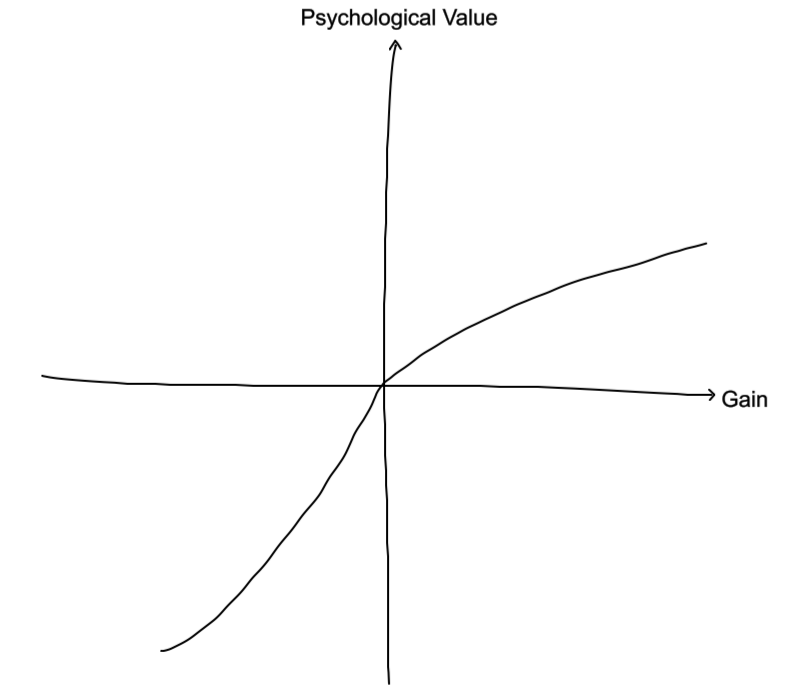
\includegraphics[width=0.6\linewidth]{prospecttheory}
\end{figure}

The reference point is not dependent on current wealth.

The slope is steeper in the loss section than the gain section -- this means
that we feel losses more keenly than gains. So humans are \textit{generally}
risk-averse.

The slope gets less steep the further away you go from the reference point.
This means that beyond a point, gain and loss feels little different.
Consider winning $\pounds 30m$ compared to winning $\pounds 100m$.
The feeling for both would be very similar despite one being over 3x as much.

\item Explain what is meant by the ``tragedy of the commons'' and how the concept 
relates to password usability.

The tragedy of the commons is when a limited and unregulated resource is shared between a group of people.
Every person then acts in their own self-interest and uses it greatly, leading to the resource being depleted or
damaged. Every new user uses up a small part of the resource, however not enough for it individually to be a problem.

The classic example is grazing sheep in a field -- one more sheep makes no difference and that
sheep gets to eat. However after a few hundred sheep there is no grass left for any sheep. Another example is
voting -- many people think ``my vote doesn't matter'' and eventually all those people who say ``my vote doesn't
matter'' make a difference. In reality those votes often can make a difference. Consider the 2000 US presidential
election where 500 votes decided the presidency.

% In relation to passwords, the shared resource is passwords. Each individual website who uses a password doesn't make
% the whole system less secure.

% The tragedy of the commons relates to password security as every website who starts using passwords thinks
% ``passwords can't be so bad since everyone else uses them''. However every new website which starts using passwords
% makes them marginally worse for every other user.

% Password security: very easy to add the same password to another account -- but when you do this it slightly
% decreases the security of every other account you've got which is also using the same password.

% Everyone uses passwords -- so they can't be too bad! But they are! The cost to support one more user is negligible.
% But one more user adding a password makes passwords as a whole less secure.

% Wrong answer:

% One person using a bad password doesn't make passwords worse or more vulnerable -- buttt, now passwords as a whole are
% less secure. And now hackers are more aware that passwords are bad and are more likely to guess ``password'' as a
% password.

\item Explain what is meant by ``compliance budget'' and how the concept relates to 
password usability.

Users have finite patience and are therefore only willing to put in a limited amount of effort into complying with
security protocols.
For example if you ask users to use strong passwords then they will use strong passwords. Or if you ask users to
change their password every 3 months then they will change their password every 3 months. However, users will not do
both as it's far too much effort. Instead users will often just add a counter on the end of a weak password
or cycle through a small set of weak passwords.

This means that the compliance budget must be managed like any other budget and system administrators and security
professionals must be careful which advice they recommend and how difficult it is to follow -- because if they
recommend too much users will simply stop following it.

\end{enumerate}

\end{examquestion}

\end{enumerate}

\end{document}
